\documentclass{article}
\usepackage{realtristan}
\title{Physics Research}
\author{Tristan Simpson}
\begin{document}
\maketitle
\tableofcontents
\section{Waves}
\subsection{Mechanical Waves}
A mechanical wave is a wave that is an \hyperref[sec:oscillation]{oscillation} of matter and is responsible for the transfer of energy through a medium. (Note: Light is not a mechanical wave because it is not matter. The particles that make up light (photons) have no mass.)

\subsubsection{Different Types of Mechanical Waves}
In total there are \textbf{three} types of mechanical waves. These waves are: Transverse Waves, Longitudinal Waves, and Combined Waves.

\subsection{Electromagnetic Waves}
Electromagnetic waves are those created by \hyperref[sec:oscillation]{oscillating} electric and magnetic fields. A great example of an electromagnetic wave is light. Light has two components: vertical and horizontal (electric and magentic field oscillation). This combination results in an electromagnetic wave.

\subsubsection{Different Types of Electromagnetic Waves}
In total there are \textbf{seven} types of electromagnetic waves. These waves are: Radio Waves, Microwaves, Infrared, Visible, Ultraviolet, X-Ray, and Gamma Rays.

\subsection{Gravitational Waves}
First proposed by Albert Einstein in 1916 following his famously recognized \hyperref[sec:generalrelativity]{Theory of General Relativity}, gravitational waves are ripples in space-time (the fabled “fabric” of the Universe) caused by massive objects moving with extreme accelerations.\\\\
In a 1936, Albert Einstein and Nathan Rosen submitted a manuscript famously claiming that gravitational waves do not exist. Gravitational waves were thought to be physically impossible. \\\\
Gravitational waves were later proved to be existent, though it was determined that they would be so weak, detecting them would be impossible. However, in 2015, the Laser Interferometer Gravitational-Wave Observatory (LIGO) detected gravitational waves from the collision of two black holes.\\\\
Gravitational waves are formed by, as an example, also described above, two black holes orbiting eachother, both getting closer and closer together until they collide.\\\\

\subsubsection{Gravitational Wave Visualization}
Gravitational waves are a very difficult concept to visualize. The following image is a basic visualization of gravitational waves. The two light-blue spheres are, for example, black holes. Their circulation around eachother leave ripples in spacetime.\\\\
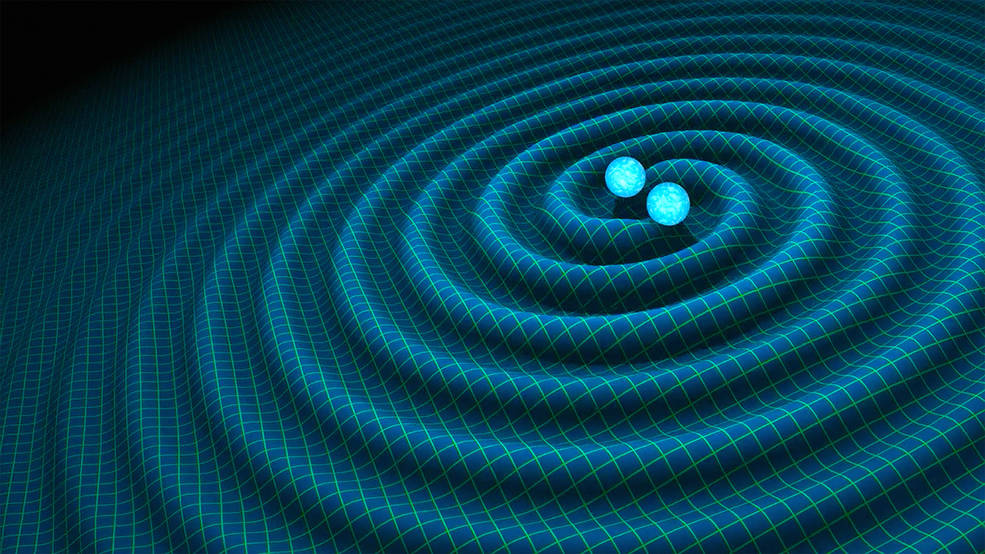
\includegraphics[scale=0.33]{images/gravitational_waves.png}

\subsection{Matter Waves}
Matter waves are a central part of the theory of quantum mechanics, being an example of wave-particle duality. All matter exhibits wave-like behavior. The matter waves describes the relationship being momentum and wavelength.


\section{Light}
\subsection{Wave Velocity}
The speed of an electromagnetic wave (therefore light waves) is dependant on the wave length and freuency. The measure of a waves velocity can be calculated by the following equation: $v = \lambda f$ where $v$ is the velocity, $\lambda$ is the wave length, and $f$ is the frequency. The units of velocity are meters per second (m/s).

\subsection{Components}
A light wave is made up of two components: electric and magnetic fields. These components can also be represented as vertical and horizontal vectors. These vectors later appear in the polarization of light waves.

\subsection{Films}
Films allow the light wave to refract and reflect along the innerds of the film. This causing the reflecting light wave (the wave hitting the screen) to either constructively or deconstructively interfere.

\subsection{Polarization}
The polarization of a light wave allows for either the vertical or horizontal components of a wave to be eliminated. This elimination removes a minimum of $50\%$ of the lights' brightness.

\subsection{Gravitational Lensing}
Following Einstein's \hyperref[sec:generalrelativity]{Theory of General Relativity}, light can be bent by gravity. This bending is known as gravitational lensing. Through gravitational lensing, lights path around the electromagnetic field of an extensively large mass (eg. a neutron star) is curved.

\subsubsection{Gravitational Micro-Lensing}
Gravitational micro-lensing allows astronomers to detect objects that would otherwise be hidden in our vast universe (ie. a black hole). To detect a black hole, taken from a discovery by astronomers in 2019, the light of a star was observed to be distorted by the gravitational lensing of a black hole.

\subsubsection{So how does it work?}
The best way to describe gravitational lensing is through the visualization of a vowling bowl circulating a pit. Because of the momentum of the bowling ball, it's doesn't just simply fall into the pit. Instead, it curves around it. (ie. light around objects of extensively large mass)

\subsection{Light - A Particle and Wave}
Not only is light a wave, but it is also a particle. This is known as wave-particle duality which is an essential theory derived from electromagnetics in quantum mechanics.

\subsubsection{Light as a Wave}
Combatting Isaac Newton's belief that light is a particle was Christiaan Huygens who had instead proposed that light was a wave. At the time Huygens wasn't able to prove his theory. It wasn't until 123 years later (1678 to 1801) that Thomas Young proved light was a wave through his Double Slit experiment.

\subsubsection{Light as a Particle}
Albert Einstein's quantum theory of light proposes that light is a series of photons (a packet of electromagnetic energy with no mass nor any charge), and the flow of photons is a wave. Einstein's essential point is that light's energy is directly related to its oscillation frequency.



\section{Planck's Constant}




\section{General Relativity}\label{sec:generalrelativity}




\section{Neutron Stars and Pulsars}




\section{Black Holes}




\section{White Holes}




\section{Worm Holes}




\section{Word Bank}
\subsection{Oscillation}\label{sec:oscillation}
The movement back and forth at a regular speed. Regular variation in magnitude or position around a central point.

\end{document}